\documentclass[conference]{IEEEtran}
\IEEEoverridecommandlockouts
% The preceding line is only needed to identify funding in the first footnote. If that is unneeded, please comment it out.
\usepackage{cite}
\usepackage{amsmath,amssymb,amsfonts}
\usepackage{algorithmic}
\usepackage{graphicx}
\usepackage{textcomp}
\usepackage{xcolor}
\usepackage{hyperref}
\usepackage{pgfplots}

\def\BibTeX{{\rm B\kern-.05em{\sc i\kern-.025em b}\kern-.08em
    T\kern-.1667em\lower.7ex\hbox{E}\kern-.125emX}}
\begin{document}

\title{Predicting and visualizing daily happiness of people using tracking data of consumer services and devices.\\
\thanks{Identify applicable funding agency here. If none, delete this.}
}

\author{

\IEEEauthorblockN{Christian Reiser}
\IEEEauthorblockA{
\textit{University of Stuttgart}\\
Stuttgart, Germany \\
christian.reiser@insightme.org}

\and

\IEEEauthorblockN{Tanja Blascheck}
\IEEEauthorblockA{
\textit{University of Stuttgart}\\
Stuttgart, Germany \\
tanja.blascheck@vis.uni-stuttgart.de}

\and

\IEEEauthorblockN{Benedikt V. Ehinger}
\IEEEauthorblockA{
\textit{University of Stuttgart}\\
Stuttgart, Germany \\
benedikt.ehinger@vis.uni-stuttgart.de}

}

\maketitle

\begin{abstract}
We offer the code for this work in open source.
\color{red}
...\\
...\\
...
\color{black}

\end{abstract}

\begin{IEEEkeywords}
machine learning, visualization, subjective well-being, mobile, quantified-self
\end{IEEEkeywords}

%=============================================================================
\section{Introduction}
We know that our environment and actions play a major role in our well-being, health, intellectual and athletic performance.
However, there is less certainty about how much our environment (e.g., weather, air quality, noise) or behavior (e.g., nutrition, exercise, meditation, sleep) influence our happiness, productivity, sports performance, or allergies.
Furthermore, on some days, we are surprised that we are less motivated, our athletic performance is poor, or the disease symptoms are more severe.

To understand ourselves better, we built a system that predicts a variable of interest like well-being from past behavior and environmental data.
The system explains the predictions by visualizing its reasoning. 

This paper focuses on daily subjective well-being and explores its associations with outdoor and indoor weather, sleep and exercise, body weight, nutrition, heart rate, screentime, and productivity.


\subsection{How is well-being defined?}
Psychologists often refer to subjective well-being (SWB) as frequent positive affect, infrequent negative affect, and cognitive evaluations of what a person considers a good life \cite{tov_subjective_2013}.

such as being enthusiastic, energetic, confident, active, and alert, optimistic, happy, joyful, curious, excited, relaxed, grateful
such as being sad, lethargic, distressed, in pain, anxious, sick, pessimistic, angry
In their review of literature on affect Barsade and Gibson (2012) define positive affectivity as the tendency of individuals to be cheerful and to experience positive moods, such as pleasure or well-being across a variety of situations, as compared to individuals who tend to be low energy and melancholy.

This study aims to test the predictive power of behavioral and sensor-based variables such as heart rate, weather, and sleep regarding subjective well-being.
To gather well-being data, we built a mobile app that asks the user to rate the days' average subjective well-being at the end of the day. 

\subsection{How is well-being measured?}
Rating in the evening before sleep:
Taking all together, how satisfied or dissatisfied were you today on a scale from one to nine?

This rating mechanism has downsides due to recency bias, leading to the greater importance of recent events and fading affect bias, where negative memories fade faster than positive ones (Skowronski, Walker, et al., 2014).
Asking for a rating multiple times per day would reduce these biases; however, we decided against it, as it requires more effort and thus is less sustainable over long periods. 



%=============================================================================

\section{Related Work}
This section provides an overview of relevant work, with a focus on (\ref{sec:wellbeing}) well-being prediction and (\ref{sec:apps}) related mobile applications.

\subsection{Prediction of well-being}
\label{sec:wellbeing}

In the last decade, affective computing stated to explore predicting mood, wellbeing, happiness and emotion from sensor data gathered through a varierty of sources.

An unimodal heartbeat time series, measured with a professional EGC device has been shown to predict emotional valence, when the participant is seated. \cite{harper_bayesian_2020}\\


Major depressive disorder can be detected with an average accuracy of ~70\% from twitter behavior, in a study of twitter users, who posted more than 4500 tweets on average\cite{choudhury_predicting_2013}.\\ 

Several studies estimated mood, stress and health with data from multimodal wearable sensors, a smartphone app, and daily manually reported behaviors such as academic activities, exercise claiming maximum accuracies of mood of
 68.48\%\cite{jaques_predicting_2015},
 74.3\%\cite{jaques_multi-task_2015},
 82.52\%\cite{jaques_multi-task_2016} all with a baseline of  53.94. Another study achieves 78.7\% with a baseline of 50.4\%\cite{taylor_personalized_2020}. 
 

The above mentioned studies might be less practical for long term every day usage as expensive professional equipment, time consuming manual reporting of activity duration or frequent social media behavior is needed.

Therefore, we focus on cheap and passive data-sources, requiring minimal attention in everyday life.

It has been shown that mood can be predicted from passive data, specifically keyboard and application data from mobile phones with a maximum accuracy of 66.59\% (62.65\% if without text) compared to a baseline of 40.18\% \cite{liu_multimodal_2020}\\


\subsection{Related Apps}
\label{sec:apps}

There are several apps which allow users to track their mood  \cite{noauthor_moodprism_nodate}\cite{noauthor_moodily_nodate} \cite{noauthor_moodpanda_nodate}\cite{noauthor_daylio_nodate} \cite{noauthor_mood_nodate}\cite{noauthor_mood_nodate-1}\cite{fitbit_stress_nodate} \cite{appleinc_ios_nodate}\cite{hellocodeinc_exist_nodate}.
Some health apps allow to correlate symptoms with food and behavior \cite{noauthor_pattern_nodate}\cite{noauthor_features_nodate}.
There is increasing development in apps predicting activity of the sympathetic nervous system from heart rate and heart rate variability \cite{welltory_welltory_nodate}\cite{elitehrv_best_nodate} which claim to estimate stress, energy, and productivity levels\cite{welltory_welltory_nodate}, or if someone should exercise harder or teak a break\cite{elitehrv_best_nodate}.
FitBit also shows a "Stress Management" score which is computed taking data about sleep, electro-dermal acticity and exercise into account\cite{fitbit_stress_nodate}.

%=============================================================================

\section{Data sources}
The aim is to use non-intrusive, inexpensive sensors and services that are robust and easy to use over a few years. 
Examples are, fitness tracker for exercise and sleep, indoor and outdoor weather stations, screentime logger, nutrition, weekday, medication.
The reader can find a list of all data sources and explanations in the Appendix.
%=============================================================================

\section{Methods}
\subsection{Pre-processing}
These data types' sampling rates vary between 5 minutes (e.g., $heart-rate$) to ~ weekly ($Bodyweight$ and $VO2Max$).

\subsubsection{Data Aggregation}
The goal is to have a sampling rate of 24h.
In most cases, the sampling rate is $>$24h, and the data is aggregated in 24h intervals by taking the sum, fifth percentile, 95th percentile, and median.
We use the fifth and 95th percentile instead of the minimum and maximum since they are less noisy and more predictive.

\subsubsection{Data Impution}
The sampling frequency of $Bodyweight$ and $VO2Max$ is usually $<$24h.
Since $Bodyweight$ and $VO2Max$ represent physical entities that change relatively slowly, we assume a linear change, allowing linear interpolation to achieve the 24h frequency.

\subsubsection{Time-series} 
\label{sec:time-series}
Since the dataset is a time series, we added all yesterday's values as features, including yesterday's well-being.

\begin{figure}[htbp]
\begin{center}
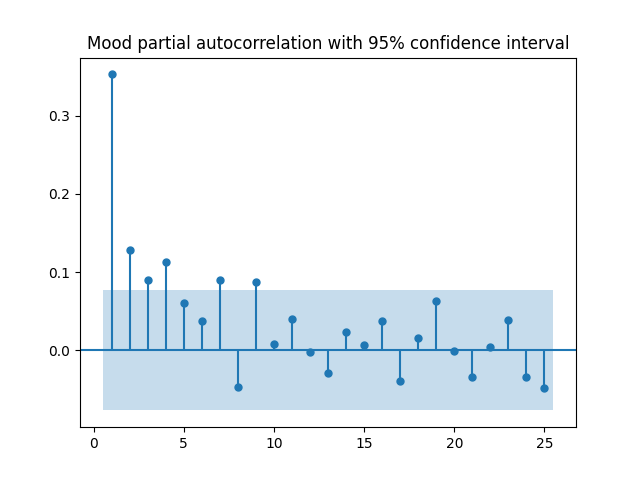
\includegraphics[width=1\linewidth]{figs/partial_autocorrelation_025lags_Mood.png}
\caption[Partial autocorrelation]{Partial autocorrelation of subjective well-being. The first data point, which represents the subjective well-being of one day ago, is considerable. The points representing the partial autocorrelation of 3 and 4 days ago are barely significant.}
\label{fig:partial_auto_corr}
\end{center}
\end{figure}


Figure \ref{fig:partial_auto_corr} shows the partial autocorrelation of well-being. Note that the first value, which represents the well-being of one day ago, is considerable, while the partial autocorrelations of 2 to 4 days ago are barely significant.

\subsection{Data Exploration}
Since the sensors and services which provide the data are cheap consumer devices, the data has many outliers.
For example, the estimated metabolic energy output, shown in figure \ref{fig:kcal_out} has values at ~1000 kcal and above 4000 kcal which are probably outliers.


\begin{figure}[htbp]
\begin{center}
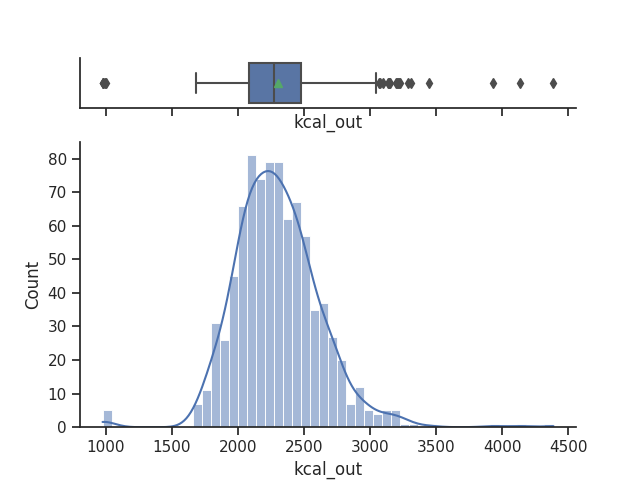
\includegraphics[width=1\linewidth]{figs/kcal_out.png}
\caption{Distribution of the estimated metabolic energy output. Values below 1600 kcal and above 3500 kcal are outliers.}
\label{fig:kcal_out}
\end{center}
\end{figure}

Moreover, figure \ref{fig:co2} shows a suspicious $CO_2$ spike at 5000 pmm. A closer look into the raw sensor data depicted in figure \ref{fig:netatmo_co2} indicates an improbable saturation at 5000 pmm. The causal explanation is an ending sensor range at 5000 ppm, which falsely counts all values greater than 5000 to 5000 ppm.

\begin{figure}[htbp]
\begin{center}
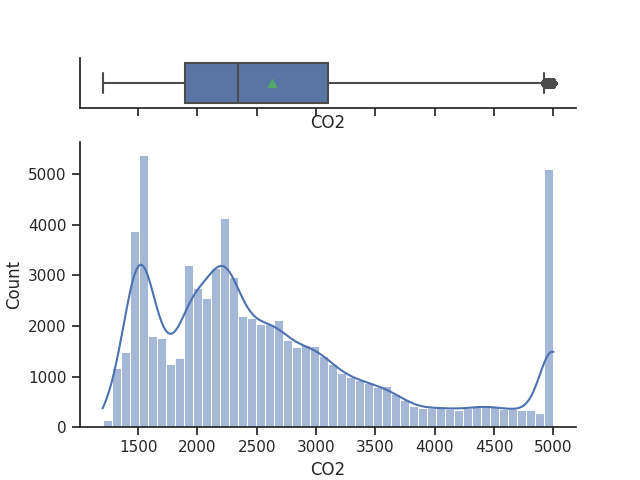
\includegraphics[width=1\linewidth]{figs/CO2.png}
\caption{Distribution of CO2 data. Note the frequent occurrence of 5000ppm as it is the sensor's maximum range.}
\label{fig:co2}
\end{center}
\end{figure}

% CO2 sensor raw data
\begin{figure}
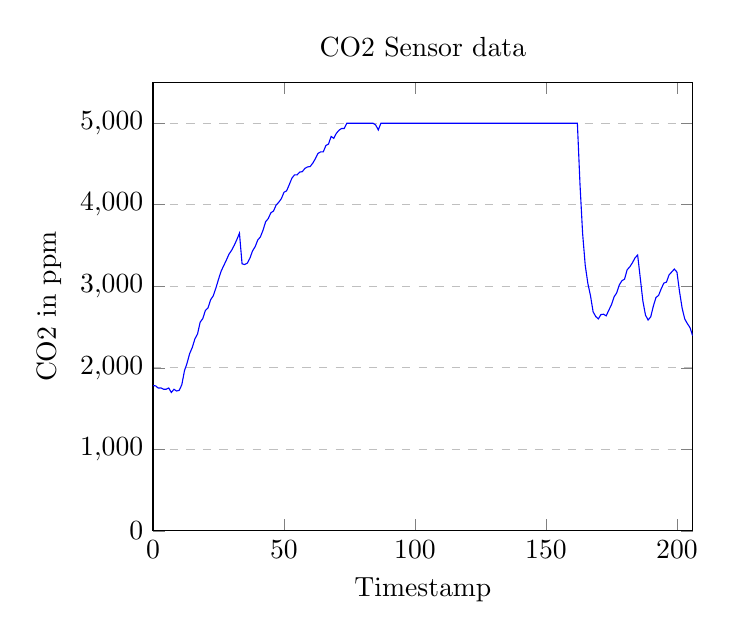
\begin{tikzpicture}
\begin{axis}[
    title={CO2 Sensor data},
    xlabel={Timestamp},
    ylabel={CO2 in ppm},
    xmin=0, xmax=206,
    ymin=0, ymax=5500,
    xtick={0,50,100,150,200},
    ytick={0,1000,2000,3000,4000,5000},
    legend pos=south west,
    ymajorgrids=true,
    grid style=dashed,
]

\addplot[
    color=blue,
    mark=none,
    ]
    coordinates {
    (0,1782)(1,1778)(2,1751)(3,1753)(4,1737)(5,1737)(6,1752)(7,1697)(8,1736)(9,1715)(10,1723)(11,1792)(12,1962)(13,2057)(14,2175)(15,2250)(16,2355)(17,2415)(18,2560)(19,2603)(20,2704)(21,2734)(22,2835)(23,2883)(24,2977)(25,3085)(26,3185)(27,3253)(28,3321)(29,3393)(30,3441)(31,3502)(32,3572)(33,3651)(34,3275)(35,3267)(36,3284)(37,3345)(38,3434)(39,3486)(40,3568)(41,3606)(42,3688)(43,3792)(44,3831)(45,3902)(46,3923)(47,3996)(48,4031)(49,4075)(50,4153)(51,4171)(52,4245)(53,4325)(54,4366)(55,4366)(56,4401)(57,4406)(58,4447)(59,4464)(60,4469)(61,4511)(62,4566)(63,4630)(64,4649)(65,4649)(66,4727)(67,4745)(68,4838)(69,4815)(70,4877)(71,4914)(72,4936)(73,4936)(74,5000)(75,5000)(76,5000)(77,5000)(78,5000)(79,5000)(80,5000)(81,5000)(82,5000)(83,5000)(84,5000)(85,4979)(86,4918)(87,5000)(88,5000)(89,5000)(90,5000)(91,5000)(92,5000)(93,5000)(94,5000)(95,5000)(96,5000)(97,5000)(98,5000)(99,5000)(100,5000)(101,5000)(102,5000)(103,5000)(104,5000)(105,5000)(106,5000)(107,5000)(108,5000)(109,5000)(110,5000)(111,5000)(112,5000)(113,5000)(114,5000)(115,5000)(116,5000)(117,5000)(118,5000)(119,5000)(120,5000)(121,5000)(122,5000)(123,5000)(124,5000)(125,5000)(126,5000)(127,5000)(128,5000)(129,5000)(130,5000)(131,5000)(132,5000)(133,5000)(134,5000)(135,5000)(136,5000)(137,5000)(138,5000)(139,5000)(140,5000)(141,5000)(142,5000)(143,5000)(144,5000)(145,5000)(146,5000)(147,5000)(148,5000)(149,5000)(150,5000)(151,5000)(152,5000)(153,5000)(154,5000)(155,5000)(156,5000)(157,5000)(158,5000)(159,5000)(160,5000)(161,5000)(162,5000)(163,4250)(164,3647)(165,3256)(166,3034)(167,2885)(168,2687)(169,2629)(170,2600)(171,2653)(172,2657)(173,2637)(174,2707)(175,2773)(176,2870)(177,2918)(178,3017)(179,3068)(180,3087)(181,3203)(182,3238)(183,3288)(184,3348)(185,3383)(186,3104)(187,2819)(188,2646)(189,2586)(190,2625)(191,2757)(192,2862)(193,2888)(194,2969)(195,3039)(196,3051)(197,3140)(198,3175)(199,3211)(200,3175)(201,2933)(202,2729)(203,2597)(204,2541)(205,2492)(206,2393)
    };

    
\end{axis}
\end{tikzpicture}
    \caption{The true CO2 level is higher than 5000 ppm but the sensors maximum is 5000 ppm.}
    \label{fig:netatmo_co2}
\end{figure}

The distribution of the wakeuptime looks gaussian except of one suspicious spice at 320 minutes after midnight. However, an alarm clock at 5:20am indicates plausibility of this spice.
% sleep end
\begin{figure}[htbp]
\begin{center}
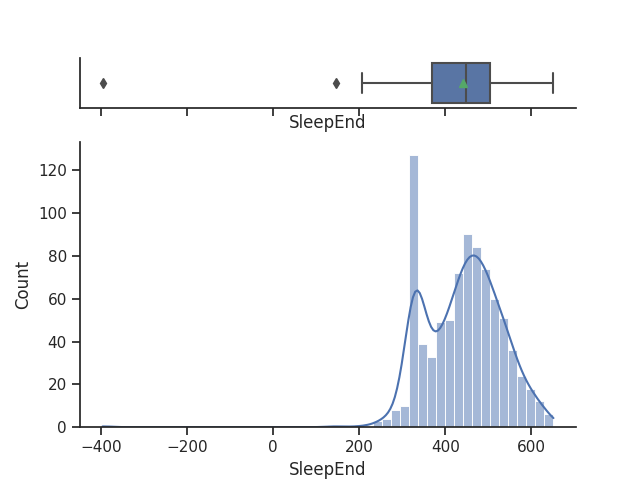
\includegraphics[width=1\linewidth]{figs/SleepEnd.png}
\caption{Wakeup time in minutes after midnight. Note the spike at 320, which is caused by the alarm clock}
\label{fig:alarm}
\end{center}
\end{figure}

Improbable values in the dataset are not corrected manually, as we don't have access to user data in the real mobile application due to privacy.
Instead we exploit robust statistics by aggregating the data via the 5th and 95th percentile instead of the maxima. Our experiments have shown that these percentiles are more predicative than maxima.


The app computes the Pearson correlation coefficient and p-Values between all attributes. Since comparing each attribute with every other, we correct the p-values according to the Benjamini-Hochberg procedure to control the false discovery rate.
A correlation is significant for p < 0.05.
Users can visually explore the data via a plotted time series with a seven-day moving average and manually inspect the relationship between two variables through scatter plots.


\subsection{Training and Hyperparamters} 
We predict well-being through multiple linear regression and a neural network. Both methods use normalized data, where each type has zero mean and unit variance.
\color{red}
TODO:\\
skip the day, interpolation, average, skip variable, multiple datasets, ensemble
\color{black}



\subsection{Train-evaluation-test-split}
Since there is a temporal dependency between observations, standard cross-validation, which assigns samples randomly to the train or test set, would lead to using some data from the future to forecast the past, which isn't possible in the real-life application. 

We use time-series-splits to avoid this fallacy. However, as only the last split uses all training data, many splits are very inefficient w.r.t. data use. Hence, we create only one split. Essentially, this is a simple train test split, where the training set contains old data points, and the test split the most recent ones.



\subsection{Multiple linear regression}
The estimation parameters for multiple linear regression (MLR) are computed via the train set while applying elastic-net regularization and sample-weighting.


\subsubsection{Regularization}
We use a combined L1 and L2 weight penalty called elastic net regularization with the formula 
\begin{equation}
\hat{\beta} \equiv \underset{\beta}{\operatorname{argmin}}\left(\|y-X \beta\|^{2}+\lambda\|\beta\|_{1}+(1-\lambda)\|\beta\|^{2}\right),
\end{equation}
with the L1 ratio $\lambda$.
Specifically, $\lambda=0$ is the ridge regularization and $\lambda=1$ is the ridge lasso regularization. We search for the optimal $\lambda$ via cross-validation.


\subsubsection{Sample-weighting}
We assume that the factors influencing a person's well-being change over time and use exponential sample-weight decay as shown in figure \ref{fig:sample-weight}.
The formula is 
\begin{equation}
sample\_weight_i = max(14.7498-13.2869(i + 30)^{0.0101585},0)
\end{equation}

which is exponential decay fitted to a value of 1 for today's datapoint and reaches zero after ~82 years. After 82 years the sample weight stays at 0 due to $max(x,0)$.
\begin{figure}[htbp]
\begin{center}
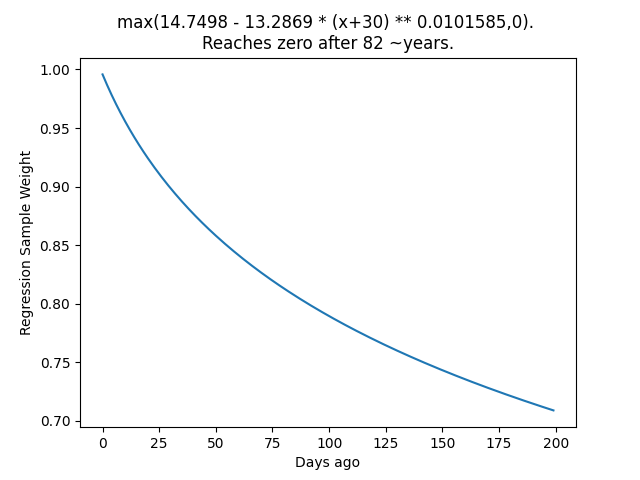
\includegraphics[width=1\linewidth]{figs/RegressionSampleWeight.png}
\caption[Sample weight]{Exponential sample-weight decay discounting older data as it might be less valuable to predict today's mood.}
\label{fig:sample-weight}
\end{center}
\end{figure}


\subsection{Neural Network}
The neural network has one fully connected hidden layer with 16 neurons followed by a Rectified Linear Unit. AdamW is the optimizer, which minimizes the mean squared error loss with a learning rate of 10e-4 and a weight decay of one. 
We searched for the best neural network architecture and hyper-parameters manually through cross-validation.


\subsection{Evaluation}
Finally, we predict well-being via the data of a previously unseen test set, record the mean squared error, and calculate the prediction intervals.

%=============================================================================

\section{Results}
Of 198 variables, 77 correlate significantly with well-being (see table \ref{tab:features} in the \ref{sec:Appendix}). Although, many of them are highly co-correlated. The principal component analysis shows in figure \ref{fig:pca} that there are only 25 components that explain more than 1\% of the variance. Examples of co-correlated variables are
\begin{itemize}
    \item all the fourfold aggregated variables (i.e., mean, median, fifth-, and 95th percentile)
    \item weather indoor and outdoor
    \item time in bed and time asleep
    \item walking minutes, heart points, exertion points
\end{itemize}

\begin{figure}[htbp]
\begin{center}
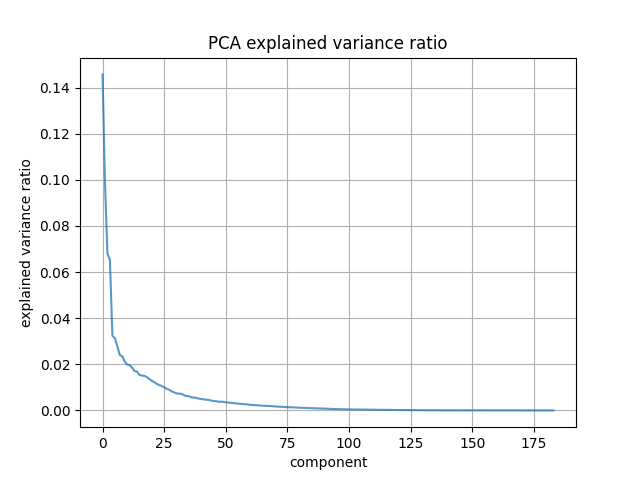
\includegraphics[width=1\linewidth]{figs/pca_explained_variance_ratio.png}
\caption{The principal component analysis shows that there are only 25 components that explain more than 1\% of the variance, indicating highly dependent features.}
\label{fig:pca}
\end{center}
\end{figure}

For prediction, we drop nutrition data, as there is only little available, reducing the number of variables to 184.

\subsection{Multiple linear regression}
Elastic-Net regularization with an L1-ration of $\lambda=1$ leads to the best prediction performance on our dataset. We interpret that feature shrinkage is more critical for generalization than reducing the L2 norm of the weights due to the high correlation of features.

\begin{table}[]
\caption[]{Regression weights. All other features have a weight of zero.}
\begin{tabular}{ll}
\textbf{Feature}       & \textbf{Regression Weight} \\
HumidInMax()           & -0.116                     \\
HeartPoints            & \,\,0.101                      \\
CO2Median()            & -0.092                     \\
MoodYesterday          & \,\,0.065                      \\
NoiseMax()Yesterday    & -0.053                     \\
PressOutMin()Yesterday & \,\,0.050                      \\
BodyWeight             & \,\,0.046                      \\
VitaminDSup            & \,\,0.032                      \\
DistractingScreentime  & -0.009                    
\end{tabular}
\label{tab:reg}
\end{table}

Table \ref{tab:reg} shows all regression weights. Note that lasso regularization selected only nine features to predict well-being. 
The prediction interval is $\pm2.3$ on the scale from 1 to 9 and $\pm1.2$ on the normalized scale with unit variance. 
\color{red}

\subsection{Neural Network}
performance.


\subsection{Explainability and Visualization}
screenshot correlation, scatter plot, p-value, \\
correlation != causality: flipping axes\\
time-series\\
prediction, interval, waterfall chart \\
Bar chart details\\
triangle details\\
A/B test\\
%=============================================================================

\section{Discussion}
L0.5-norm regularization\\
causal inference\\
explainability vs. accuracy of prediction results\\

\subsection{Limitations}


\subsection{Future Work}
 Multimodal Autoencoder: A Deep Learning Approach to Filling In Missing Sensor Data and Enabling Better Mood Prediction\cite{jaques_multimodal_2017}//
 when forcasting the mood of the next day with an mean absolute error of 17.42 while the mood standard deviation is 17.14\cite{umematsu_forecasting_2020}

\subsection{Conclusion}
1. Recap what you did. In about one paragraph recap what your research question was and how you tackled it.
2. Highlight the big accomplishments. Spend another paragraph explaining the highlights of your results. These are the main results you want the reader to remember after they put down the paper, so ignore any small details.
3. Conclude. Finally, finish off with a sentence or two that wraps up your paper. I find this can often be the hardest part to write. You want the paper to feel finished after they read these. One way to do this, is to try and tie your research to the “real world.” Can you somehow relate how your research is important outside of academia? Or, if your results leave you with a big question, finish with that. Put it out there for the reader to think about to.


\color{black}

%Backmatter
%=============================================================================

\bibliographystyle{IEEEtran}
\bibliography{refs}


%=============================================================================

\section{Appendix}
\label{sec:Appendix}

Data sources are:
\begin{itemize}
\item Moon Illumination
\item daytime (the time between sunrise and sunset, which is short er in the fall/winter and longer in the spring/summer)
\item OpenWeatherMap, which gives outside weather measurements GPS location 
   \begin{itemize}
\item temperature
\item heat index (human-perceived equivalent temperature, which includes humidity and windspeed)
\item air pressure
\item humidity
\item windspeed
\item cloud cover
\item precipitation (rain, snow)
\end{itemize}
\item Phone Location
   \begin{itemize}
\item longitude
\item latitude
\end{itemize}
\item Day of the week (Monday, Tuesday, etc.)
\item the severity of covid lockdown measures
\item commits on GitHub
\item Google Fit
   \begin{itemize}
\item Heart Points (duration and intensity exercise estimate)
\item walking minutes
\item running minutes
\item meditating minutes
\item Sleep efficiency
\item Sleep starting time
\item sleep end time
\item minutes in bed
\item minutes asleep
\item binary: was a nap taken?
\item minutes of light sleep
\item minutes of deep sleep
\item minutes of REM sleep
\item minutes awake in bed
\end{itemize}
\item Fitbit Charge 3 Smartwatch, which estimate:
   \begin{itemize}
\item steps taken
\item burned calories
\item heart rate
\item resting heart rate
\item VO2Max (maximum rate of oxygen consumption)
\item sleep revitalization
\item sleep duration score
\item sleep restlessness
\item vertical meters exercised (measured in floors)
\end{itemize}
\item Later Upgrade to Fitbit Sense Smartwatch, which extends the following estimates:
   \begin{itemize}
\item Responsiveness points: a proprietary assessment of how well the sympathetic and parasympathetic nervous system are in balance which takes Heart Rate Variability (HRV), Elevated Resting Heart Rate (RHR), Sleeping Heart Rate above RHR, and Electrodermal Activity (EDA) into account
\item Exertion points (similar to heart points)
\item the temperature of the wrist during sleep
\item sleep points (sleep rating)
\item stress points (average of sleep-, exertion-, and responsiveness points)
\end{itemize}
\item Netatmo indoor weather station
   \begin{itemize}
\item Temperature
\item Humidity
\item CO2 in ppm
\item Noise in dB
\item air pressure in Pa
\end{itemize}
\item Nutrition tracking with MyFitessPal
   \begin{itemize}
\item Carbohydrates intake
\item Fat intake
\item Protein intake
\item Sodium intake
\item fiber intake
\item sugar intake
\item cholesterol intake
\item total calories intake
\end{itemize}
\item Bodyweight (Renpho Scale) 
\item Screentime tracking, with RescueTime
   \begin{itemize}
\item total screen time
\item productive screentime
\item distracting screen time
\item neutral screen time
\end{itemize}
\end{itemize}

\begin{table}[]
\caption[]{Correlation coefficients, Benjamini–Hochberg corrected p-values and regression weights of all features. Sorted by p-values, which are bold when below 0.5.}
\label{tab:features}

\begin{tabular}{llll}
\textbf{feature} & \textbf{corr. coeff.} & \textbf{p-value} & \textbf{reg. weight} \\
MoodYesterday                  & 0.348  & \textbf{3.3E-18} & \textbf{0.06}  \\
HumidInMax()                   & -0.406 & \textbf{4.6E-09} & \textbf{-0.12} \\
BodyWeight                     & 0.248  & \textbf{4.6E-09} & \textbf{0.05}  \\
MoodEreyesterday               & 0.236  & \textbf{2.9E-08} & 0.00           \\
BodyWeightYesterday            & 0.235  & \textbf{3.0E-08} & 0.00           \\
Covid\_lifestyleYesterday      & 0.211  & \textbf{1.1E-06} & 0.00           \\
Covid\_lifestyle               & 0.210  & \textbf{1.1E-06} & 0.00           \\
HumidInMedian()                & -0.342 & \textbf{1.4E-06} & 0.00           \\
HumidInMax()Yesterday          & -0.329 & \textbf{4.2E-06} & 0.00           \\
CO2Median()                    & -0.321 & \textbf{7.3E-06} & \textbf{-0.09} \\
HumidOutMin()Yesterday         & -0.186 & \textbf{2.2E-05} & 0.00           \\
NoiseMax()Yesterday            & -0.303 & \textbf{2.9E-05} & \textbf{-0.05} \\
TempInMedian()                 & -0.301 & \textbf{3.0E-05} & 0.00           \\
HumidOutMean()Yesterday        & -0.181 & \textbf{3.3E-05} & 0.00           \\
HumidOutMax()Yesterday         & -0.179 & \textbf{3.8E-05} & 0.00           \\
HumidOutMin()                  & -0.177 & \textbf{5.1E-05} & 0.00           \\
NoiseMax()                     & -0.288 & \textbf{6.8E-05} & 0.00           \\
Daytime                        & 0.172  & \textbf{8.1E-05} & 0.00           \\
DaytimeYesterday               & 0.171  & \textbf{8.1E-05} & 0.00           \\
TempOutMax()Yesterday          & 0.171  & \textbf{8.7E-05} & 0.00           \\
HumidOutMean()                 & -0.168 & \textbf{1.2E-04} & 0.00           \\
HumidInMedian()Yesterday       & -0.276 & \textbf{1.4E-04} & 0.00           \\
TempInMax()                    & -0.270 & \textbf{2.0E-04} & 0.00           \\
HumidOutMax()                  & -0.162 & \textbf{2.0E-04} & 0.00           \\
TempOutMean()Yesterday         & 0.160  & \textbf{2.4E-04} & 0.00           \\
TempOutMax()                   & 0.157  & \textbf{3.2E-04} & 0.00           \\
HRMean()Yesterday              & -0.155 & \textbf{3.8E-04} & 0.00           \\
TempInMax()Yesterday           & -0.258 & \textbf{3.8E-04} & 0.00           \\
HumidInMin()                   & -0.257 & \textbf{3.8E-04} & 0.00           \\
TempInMedian()Yesterday        & -0.250 & \textbf{6.2E-04} & 0.00           \\
TempOutMean()                  & 0.148  & \textbf{7.8E-04} & 0.00           \\
TempFeelOutMax()Yesterday      & 0.147  & \textbf{7.8E-04} & 0.00           \\
TempFeelOutMax()               & 0.145  & \textbf{9.6E-04} & 0.00           \\
TempInMin()                    & -0.240 & \textbf{1.0E-03} & 0.00           \\
VitaminDSupYesterday           & 0.144  & \textbf{1.0E-03} & 0.00           \\
VitaminDSup                    & 0.143  & \textbf{1.1E-03} & \textbf{0.03}  \\
TempOutFeelMean()Yesterday     & 0.142  & \textbf{1.1E-03} & 0.00           \\
PressureInMin()Yesterday       & 0.234  & \textbf{1.3E-03} & 0.00           \\
TempOutFeelMean()              & 0.134  & \textbf{2.5E-03} & 0.00           \\
TempOutDelta()Yesterday        & 0.133  & \textbf{2.6E-03} & 0.00           \\
CO2Max()                       & -0.220 & \textbf{2.8E-03} & 0.00           \\
PressureInMedian()Yesterday    & 0.221  & \textbf{2.8E-03} & 0.00           \\
Fiber                          & 0.195  & \textbf{3.6E-03} &                \\
TempFeelOutMin()Yesterday      & 0.129  & \textbf{3.8E-03} & 0.00           \\
TempOutMin()Yesterday          & 0.127  & \textbf{4.5E-03} & 0.00           \\
PressureInMax()Yesterday       & 0.209  & \textbf{4.9E-03} & 0.00           \\
FiberYesterday                 & 0.188  & \textbf{5.3E-03} &                \\
TempOutDelta()                 & 0.124  & \textbf{5.3E-03} & 0.00           \\
SleepRevitalizationYesterday   & 0.123  & \textbf{6.3E-03} & 0.00           \\
HeartPoints                    & 0.121  & \textbf{6.6E-03} & \textbf{0.10}  \\
HighLongitude                  & 0.120  & \textbf{6.6E-03} & 0.00           \\
CO2Min()                       & -0.199 & \textbf{7.0E-03} & 0.00           \\
CO2Median()Yesterday           & -0.199 & \textbf{7.2E-03} & 0.00           \\
TempFeelOutMin()               & 0.117  & \textbf{8.6E-03} & 0.00           \\
SleepLight                     & -0.117 & \textbf{8.6E-03} & 0.00           \\
HumidInMin()Yesterday          & -0.194 & \textbf{8.9E-03} & 0.00           \\
TempOutMin()                   & 0.115  & \textbf{9.2E-03} & 0.00           \\
CloudOutMean()                 & -0.114 & \textbf{1.0E-02} & 0.00           \\
CloudOutMean()Yesterday        & -0.114 & \textbf{1.0E-02} & 0.00           \\
CloudOutMax()Yesterday         & -0.113 & \textbf{1.1E-02} & 0.00           \\
NoiseMedian()Yesterday         & -0.188 & \textbf{1.1E-02} & 0.00           \\
TempInMin()Yesterday           & -0.185 & \textbf{1.3E-02} & 0.00           \\
NoiseMedian()                  & -0.182 & \textbf{1.4E-02} & 0.00           \\
StressManagement               & 0.179  & \textbf{1.5E-02} & 0.00           \\
CO2Max()Yesterday              & -0.181 & \textbf{1.5E-02} & 0.00           \\
DistractingScreentimeYesterday & 0.110  & \textbf{1.5E-02} & 0.00           \\
PressureInMin()                & 0.174  & \textbf{2.0E-02} & 0.00           \\
LowLongitude                   & 0.103  & \textbf{2.2E-02} & 0.00           \\
ExertionPointsYesterday        & 0.169  & \textbf{2.2E-02} & 0.00           \\
PressureInMedian()             & 0.165  & \textbf{2.9E-02} & 0.00           \\
CarbsYesterday                 & 0.149  & \textbf{2.9E-02} &                \\
\end{tabular}
\end{table}
\begin{table}[]
\begin{tabular}{llll}
\textbf{feature} & \textbf{corr. coeff.} & \textbf{p-value} & \textbf{reg. weight} \\
CO2Min()Yesterday              & -0.164 & \textbf{3.0E-02} & 0.00           \\
SleepDeep                      & 0.094  & \textbf{3.8E-02} & 0.00           \\
PressureInMax()                & 0.153  & \textbf{4.6E-02} & 0.00           \\
HighLongitudeYesterday         & 0.089  & 5.4E-02          & 0.00           \\
SleepStartYesterday            & -0.089 & 5.4E-02          & 0.00           \\
HRResting                      & -0.085 & 6.5E-02          & 0.00           \\
CloudOutMax()                  & -0.084 & 7.2E-02          & 0.00           \\
RunningMin                     & 0.082  & 7.8E-02          & 0.00           \\
LowLongitudeYesterday          & 0.082  & 7.8E-02          & 0.00           \\
SleepPoints                    & 0.134  & 8.3E-02          & 0.00           \\
ScreentimeYesterday            & 0.083  & 8.3E-02          & 0.00           \\
StressManagementYesterday      & 0.131  & 9.0E-02          & 0.00           \\
NeutralScreentimeYesterday     & 0.080  & 9.5E-02          & 0.00           \\
SodiumYesterday                & 0.118  & 9.6E-02          &                \\
SleepRevitalization            & 0.077  & 1.1E-01          & 0.00           \\
Sodium                         & 0.113  & 1.2E-01          &                \\
HRMax()                        & 0.072  & 1.3E-01          & 0.00           \\
SleepLightYesterday            & -0.072 & 1.4E-01          & 0.00           \\
LowLatitude                    & -0.071 & 1.4E-01          & 0.00           \\
RunningMinYesterday            & 0.071  & 1.4E-01          & 0.00           \\
ExertionPoints                 & 0.108  & 1.8E-01          & 0.00           \\
SugarYesterday                 & 0.099  & 1.8E-01          &                \\
HRMax()Yesterday               & 0.065  & 1.9E-01          & 0.00           \\
CloudOutMin()                  & -0.065 & 1.9E-01          & 0.00           \\
Steps                          & 0.060  & 2.4E-01          & 0.00           \\
SleepWake                      & -0.060 & 2.4E-01          & 0.00           \\
SleepEndYesterday              & 0.059  & 2.5E-01          & 0.00           \\
SleepREM                       & 0.056  & 2.8E-01          & 0.00           \\
MeditatingMinYesterday         & 0.056  & 2.9E-01          & 0.00           \\
Floors                         & 0.056  & 2.9E-01          & 0.00           \\
KCalIn                         & 0.083  & 2.9E-01          &                \\
HRMin()Yesterday               & -0.054 & 3.0E-01          & 0.00           \\
SleepREMYesterday              & 0.052  & 3.3E-01          & 0.00           \\
RainSnowYesterday              & -0.051 & 3.4E-01          & 0.00           \\
PressOutDelta()Yesterday       & -0.051 & 3.4E-01          & 0.00           \\
MeditatingMin                  & 0.050  & 3.5E-01          & 0.00           \\
InBedMin                       & -0.050 & 3.5E-01          & 0.00           \\
HRRestingYesterday             & -0.050 & 3.5E-01          & 0.00           \\
HRMin()                        & -0.048 & 3.8E-01          & 0.00           \\
Sunday                         & 0.047  & 3.9E-01          & 0.00           \\
SaturdayYesterday              & 0.047  & 3.9E-01          & 0.00           \\
Carbs                          & 0.069  & 4.0E-01          &                \\
Saturday                       & -0.044 & 4.2E-01          & 0.00           \\
FridayYesterday                & -0.044 & 4.2E-01          & 0.00           \\
SleepStart                     & -0.043 & 4.3E-01          & 0.00           \\
SleepEfficiencyYesterday       & -0.043 & 4.3E-01          & 0.00           \\
SleepWakeYesterday             & -0.043 & 4.3E-01          & 0.00           \\
NoiseMin()Yesterday            & 0.071  & 4.4E-01          & 0.00           \\
PressOutDelta()                & -0.042 & 4.4E-01          & 0.00           \\
CloudOutMin()Yesterday         & -0.041 & 4.5E-01          & 0.00           \\
HeartPointsYesterday           & 0.041  & 4.5E-01          & 0.00           \\
PressOutMin()Yesterday         & 0.041  & 4.5E-01          & \textbf{0.05}  \\
HighLatitude                   & -0.041 & 4.5E-01          & 0.00           \\
NoiseMin()                     & 0.068  & 4.5E-01          & 0.00           \\
ProductiveScreentimeYesterday  & 0.041  & 4.6E-01          & 0.00           \\
ProteinYesterday               & 0.060  & 4.6E-01          &                \\
ResponsivenessPoints           & 0.065  & 4.6E-01          & 0.00           \\
LowLatitudeYesterday           & -0.039 & 4.6E-01          & 0.00           \\
WindOutMean()Yesterday         & 0.039  & 4.6E-01          & 0.00           \\
InBedMinYesterday              & -0.039 & 4.6E-01          & 0.00           \\
FatYesterday                   & -0.058 & 4.7E-01          &                \\
KcalOut                        & 0.038  & 4.7E-01          & 0.00           \\
Monday                         & -0.037 & 4.7E-01          & 0.00           \\
SundayYesterday                & -0.037 & 4.7E-01          & 0.00           \\
WindOutMin()Yesterday          & -0.037 & 4.7E-01          & 0.00           \\
HRMean()                       & -0.037 & 4.7E-01          & 0.00           \\
Cholesterol                    & 0.056  & 4.7E-01          &                \\
AsleepMin                      & -0.035 & 5.0E-01          & 0.00           \\
NeutralScreentime              & 0.035  & 5.1E-01          & 0.00           \\
KCalInYesterday                & 0.052  & 5.2E-01          &                \\
Sugar                          & 0.051  & 5.2E-01          &                \\
DistractingScreentime          & 0.034  & 5.2E-01          & \textbf{-0.01} \\
VO2MaxYesterday                & 0.034  & 5.2E-01          & 0.00           \\
RainSnow                       & -0.033 & 5.2E-01          & 0.00           \\
Fat                            & 0.050  & 5.2E-01          &                \\
KcalOutYesterday               & -0.032 & 5.3E-01          & 0.00           \\
\end{tabular}
\end{table}
\begin{table}[]
\begin{tabular}{llll}
\textbf{feature} & \textbf{corr. coeff.} & \textbf{p-value} & \textbf{reg. weight} \\
PressOutMean()Yesterday        & 0.032  & 5.3E-01          & 0.00           \\
VO2Max                         & 0.030  & 5.7E-01          & 0.00           \\
CommitsYesterday               & -0.030 & 5.7E-01          & 0.00           \\
WalkingMinYesterday            & -0.029 & 5.8E-01          & 0.00           \\
SleepRestless                  & 0.029  & 5.9E-01          & 0.00           \\
AsleepMinYesterday             & -0.027 & 6.2E-01          & 0.00           \\
SleepDeepYesterday             & 0.026  & 6.4E-01          & 0.00           \\
StepsYesterday                 & -0.025 & 6.4E-01          & 0.00           \\
Protein                        & 0.037  & 6.5E-01          &                \\
CholesterolYesterday           & 0.036  & 6.6E-01          &                \\
PressOutMax()Yesterday         & 0.022  & 6.9E-01          & 0.00           \\
SleepEfficiency                & 0.022  & 6.9E-01          & 0.00           \\
Commits                        & 0.022  & 6.9E-01          & 0.00           \\
Screentime                     & 0.022  & 6.9E-01          & 0.00           \\
SleepPointsYesterday           & 0.035  & 6.9E-01          & 0.00           \\
WindOutMax()Yesterday          & 0.021  & 7.0E-01          & 0.00           \\
SleepDurationScore             & 0.021  & 7.0E-01          & 0.00           \\
PressOutMin()                  & 0.020  & 7.1E-01          & 0.00           \\
TempWristNight                 & 0.031  & 7.3E-01          & 0.00           \\
HighLatitudeYesterday          & -0.018 & 7.3E-01          & 0.00           \\
WindOutMean()                  & 0.018  & 7.4E-01          & 0.00           \\
SleepDurationScoreYesterday    & 0.018  & 7.5E-01          & 0.00           \\
Thursday                       & 0.017  & 7.5E-01          & 0.00           \\
WednesdayYesterday             & 0.017  & 7.5E-01          & 0.00           \\
ThursdayYesterday              & 0.015  & 7.8E-01          & 0.00           \\
Friday                         & 0.015  & 7.8E-01          & 0.00           \\
WindOutMin()                   & -0.012 & 8.4E-01          & 0.00           \\
WalkingMin                     & 0.012  & 8.4E-01          & 0.00           \\
ProductiveScreentime           & 0.011  & 8.6E-01          & 0.00           \\
SleepRestlessYesterday         & 0.010  & 8.6E-01          & 0.00           \\
FloorsYesterday                & 0.010  & 8.7E-01          & 0.00           \\
TempWristNightYesterday        & 0.015  & 8.8E-01          & 0.00           \\
PressOutMean()                 & 0.009  & 8.8E-01          & 0.00           \\
MondayYesterday                & 0.008  & 8.8E-01          & 0.00           \\
Tuesday                        & 0.008  & 8.8E-01          & 0.00           \\
MoonIlluminationYesterday      & 0.007  & 9.0E-01          & 0.00           \\
MoonIllumination               & 0.006  & 9.1E-01          & 0.00           \\
Wednesday                      & -0.006 & 9.1E-01          & 0.00           \\
TuesdayYesterday               & -0.006 & 9.1E-01          & 0.00           \\
SleepEnd                       & -0.005 & 9.2E-01          & 0.00           \\
WindOutMax()                   & 0.004  & 9.5E-01          & 0.00           \\
PressOutMax()                  & 0.003  & 9.5E-01          & 0.00           \\
NapYesterday                   & 0.002  & 9.8E-01          & 0.00           \\
Nap                            & 0.000  & 9.9E-01          & 0.00           \\
ResponsivenessPointsYesterday  & 0.001  & 9.9E-01          & 0.00          
\end{tabular}
\end{table}



\end{document}
